\chapter{Unified Modeling Language (UML): Structural Diagram}

\section{Pendahuluan}
UML (Unified Modeling Language) adalah bahasa pemodelan yang digunakan untuk mendeskripsikan, merancang, dan mendokumentasikan sistem perangkat lunak. UML menyediakan berbagai jenis diagram yang dikategorikan menjadi diagram struktural dan diagram perilaku. Pada chapter ini, akan dibahas diagram struktural dalam UML.

Diagram struktural digunakan untuk menggambarkan bagian-bagian statis dari suatu sistem perangkat lunak. Diagram ini menunjukkan bagaimana kelas, objek, dan komponen lainnya disusun dalam sistem.


\section{Unified Modeling Language (UML) dan Sejarahnya}

Unified Modeling Language (UML) adalah standar pemodelan visual yang digunakan dalam rekayasa perangkat lunak untuk mendeskripsikan, merancang, dan mendokumentasikan sistem perangkat lunak. UML menyediakan sekumpulan diagram yang membantu pengembang dalam memahami struktur dan perilaku sistem sebelum implementasi.

\subsection{Sejarah UML}

UML dikembangkan pada pertengahan tahun 1990-an sebagai hasil dari penggabungan berbagai metode pemodelan perangkat lunak yang telah ada sebelumnya. Sebelum UML, terdapat beberapa metode pemodelan yang digunakan secara luas, seperti:
\begin{itemize}
	\item \textbf{Booch Method} – Dikembangkan oleh Grady Booch, metode ini digunakan untuk analisis dan desain sistem berbasis objek.
	\item \textbf{Object Modeling Technique (OMT)} – Dikembangkan oleh James Rumbaugh, metode ini berfokus pada pemodelan sistem berbasis objek dengan berbagai perspektif.
	\item \textbf{Object-Oriented Software Engineering (OOSE)} – Dikembangkan oleh Ivar Jacobson, metode ini memperkenalkan konsep \textit{use case} dalam pengembangan perangkat lunak.
\end{itemize}

Pada tahun 1994, Grady Booch, James Rumbaugh, dan Ivar Jacobson mulai bekerja sama untuk mengembangkan standar pemodelan terpadu. Mereka dikenal sebagai \textbf{Three Amigos} dalam dunia rekayasa perangkat lunak. Upaya mereka menghasilkan versi awal UML yang kemudian diserahkan kepada Object Management Group (OMG) pada tahun 1997 untuk standarisasi.

\subsection{Perkembangan UML}
Setelah disetujui oleh OMG, UML terus berkembang dengan berbagai revisi dan penyempurnaan. Beberapa tonggak penting dalam perkembangan UML meliputi:
\begin{itemize}
	\item \textbf{UML 1.0 (1997)} – Versi pertama yang distandarisasi oleh OMG.
	\item \textbf{UML 1.3 (1999)} – Peningkatan dalam elemen diagram dan dukungan lebih baik untuk pengembangan perangkat lunak berbasis objek.
	\item \textbf{UML 2.0 (2005)} – Pembaruan besar yang mencakup lebih banyak jenis diagram, seperti \textit{interaction overview diagram} dan peningkatan dalam ekspresi perilaku sistem.
	\item \textbf{UML versi terbaru} – UML terus diperbarui oleh OMG untuk mendukung perkembangan teknologi perangkat lunak.
\end{itemize}

\subsection{Penerapan UML dalam Rekayasa Perangkat Lunak}
Saat ini, UML digunakan secara luas dalam berbagai bidang rekayasa perangkat lunak, termasuk:
\begin{itemize}
	\item Pengembangan sistem berbasis objek.
	\item Pemodelan arsitektur perangkat lunak dan sistem berbasis layanan (\textit{service-oriented architecture}).
	\item Perancangan basis data dan sistem terdistribusi.
	\item Dokumentasi proyek perangkat lunak secara formal.
\end{itemize}

UML telah menjadi standar industri dalam pemodelan perangkat lunak dan digunakan oleh perusahaan besar serta komunitas akademik untuk meningkatkan pemahaman sistem sebelum diimplementasikan.


\section{Tools Pemodelan Perangkat Lunak}

Pemodelan perangkat lunak adalah proses penting dalam rekayasa perangkat lunak yang memungkinkan pengembang untuk mendokumentasikan, merancang, dan memahami sistem sebelum implementasi. Pemodelan ini biasanya dilakukan menggunakan berbagai alat bantu (\textit{tools}) yang mendukung pembuatan diagram UML (Unified Modeling Language). Beberapa tools yang umum digunakan dalam pemodelan perangkat lunak antara lain:

\begin{itemize}
	\item \textbf{Enterprise Architect} – Alat profesional yang mendukung pemodelan berbasis UML, digunakan untuk dokumentasi dan analisis arsitektur perangkat lunak.
	\item \textbf{StarUML} – Alat open-source untuk pemodelan berbasis UML dengan antarmuka grafis yang interaktif.
	\item \textbf{Visual Paradigm} – Mendukung pemodelan berbagai diagram UML dengan fitur analisis dan dokumentasi yang kuat.
	\item \textbf{Draw.io} – Alat berbasis web untuk membuat berbagai diagram, termasuk UML.
	\item \textbf{PlantUML} – Alat pemodelan berbasis teks yang memungkinkan pembuatan diagram UML menggunakan skrip sederhana.
\end{itemize}

\subsection{PlantUML sebagai Alat Pemodelan Berbasis Teks}

\textbf{PlantUML} adalah alat pemodelan yang memungkinkan pengguna untuk membuat diagram UML menggunakan sintaks berbasis teks. Berbeda dengan alat lain yang menggunakan antarmuka grafis, PlantUML menggunakan pendekatan deklaratif di mana diagram dibuat dengan menuliskan kode dalam format teks yang kemudian dirender menjadi diagram visual.

\subsubsection{Keunggulan PlantUML}
Beberapa keunggulan yang membuat PlantUML banyak digunakan dalam pemodelan perangkat lunak adalah:
\begin{itemize}
	\item \textbf{Berbasis Teks} – Diagram dapat dibuat dengan kode sederhana yang dapat dengan mudah diintegrasikan dalam sistem kontrol versi seperti Git.
	\item \textbf{Mendukung Berbagai Jenis Diagram} – PlantUML dapat digunakan untuk membuat diagram UML seperti \textit{class diagram}, \textit{sequence diagram}, \textit{component diagram}, \textit{object diagram}, dan lainnya.
	\item \textbf{Integrasi dengan Berbagai Platform} – PlantUML dapat digunakan di berbagai editor seperti VS Code, IntelliJ IDEA, Eclipse, serta dapat diintegrasikan dengan dokumen LaTeX dan Markdown.
	\item \textbf{Ringan dan Mudah Digunakan} – Tidak memerlukan antarmuka grafis, cukup menuliskan skrip dalam format teks.
\end{itemize}

\section{Instalasi dan Penggunaan PlantUML}

PlantUML adalah alat berbasis teks yang digunakan untuk membuat diagram UML dengan cara yang cepat dan efisien. Diagram dapat dibuat dengan mendefinisikan struktur dalam format teks menggunakan sintaks yang sederhana. PlantUML dapat digunakan dalam berbagai cara, baik secara online maupun melalui integrasi dengan editor seperti Visual Studio Code.

\subsection{Menggunakan PlantUML Secara Online}

PlantUML menyediakan layanan \textbf{online editor} yang memungkinkan pengguna membuat diagram tanpa perlu menginstal perangkat lunak tambahan. Berikut langkah-langkah untuk menggunakannya secara online:

\begin{enumerate}
	\item Buka situs resmi PlantUML di \url{https://www.plantuml.com/plantuml/uml/}.
	\item Ketik atau tempel kode diagram PlantUML ke dalam editor yang tersedia.
	\item Klik tombol \textbf{Submit} atau gunakan kombinasi keyboard \texttt{Ctrl + Enter} untuk melihat hasil diagram.
	\item Diagram dapat diunduh dalam format PNG atau SVG dengan mengklik tombol \textbf{Download}.
\end{enumerate}

Situs ini cocok digunakan bagi pengguna yang ingin mencoba PlantUML tanpa harus melakukan instalasi di komputer.

\subsection{Menggunakan PlantUML di Visual Studio Code}

Untuk pengguna yang ingin mengintegrasikan PlantUML dengan Visual Studio Code, berikut langkah-langkah instalasinya:

\subsubsection{1. Instalasi Plugin PlantUML}
\begin{enumerate}
	\item Buka Visual Studio Code.
	\item Klik menu \textbf{Extensions} atau tekan \texttt{Ctrl + Shift + X}.
	\item Cari ekstensi \textbf{PlantUML} oleh \textit{jebbs}.
	\item Klik \textbf{Install} untuk menginstal ekstensi tersebut.
\end{enumerate}

\subsubsection{2. Instalasi Java dan Graphviz (Opsional)}
PlantUML memerlukan \textbf{Java} untuk berjalan secara lokal. Untuk memastikan kompatibilitas, lakukan langkah berikut:
\begin{enumerate}
	\item Unduh dan instal Java JDK dari \url{https://www.oracle.com/java/technologies/javase-jdk11-downloads.html}.
	\item Tambahkan Java ke dalam variabel lingkungan sistem (\texttt{JAVA\_HOME}).
	\item Unduh dan instal \textbf{Graphviz} dari \url{https://graphviz.gitlab.io/download/} jika ingin meningkatkan kualitas rendering diagram.
\end{enumerate}

\subsubsection{3. Membuat dan Menjalankan Diagram PlantUML di VS Code}
Setelah ekstensi berhasil dipasang, pengguna dapat mulai membuat diagram:
\begin{enumerate}
	\item Buat file baru dengan ekstensi \texttt{.puml}, misalnya \texttt{diagram.puml}.
	\item Tambahkan kode diagram berikut sebagai contoh:
	\begin{lstlisting}[language=puml]
		@startuml
		Alice -> Bob: Hello Bob!
		Bob --> Alice: Hi Alice!
		@enduml
	\end{lstlisting}
	\item Untuk melihat pratinjau diagram, tekan \texttt{Alt + D} atau gunakan perintah \texttt{PlantUML: Preview Current Diagram}.
	\item Diagram akan langsung ditampilkan dalam jendela pratinjau di VS Code.
\end{enumerate}

\subsection{Export Diagram PlantUML}
PlantUML mendukung berbagai format ekspor, termasuk \textbf{PNG, SVG, EPS, dan PDF}. Diagram dapat diekspor menggunakan perintah:

\begin{lstlisting}[language=bash]
	java -jar plantuml.jar -tpng diagram.puml
	java -jar plantuml.jar -tsvg diagram.puml
\end{lstlisting}

Untuk pengguna \textbf{VS Code}, diagram dapat diekspor langsung dengan klik kanan pada diagram dan memilih \textbf{Export Diagram}.

PlantUML adalah alat yang fleksibel untuk membuat diagram UML dengan cepat menggunakan teks. Pengguna dapat memilih antara menggunakan \textbf{editor online} atau \textbf{plugin VS Code} untuk membuat diagram sesuai kebutuhan. Dengan sintaks sederhana dan dukungan berbagai format ekspor, PlantUML menjadi solusi yang efisien untuk mendokumentasikan sistem perangkat lunak secara visual.

\section{Class Diagram}

Class diagram merupakan salah satu diagram struktural dalam Unified Modeling Language (UML) yang digunakan untuk merepresentasikan struktur statis dari suatu sistem perangkat lunak. Diagram ini menggambarkan hubungan antar kelas serta atribut dan metode yang dimiliki oleh masing-masing kelas. Berikut adalah fitur-fitur utama dalam class diagram:

\begin{figure}[ht]
	\centering
	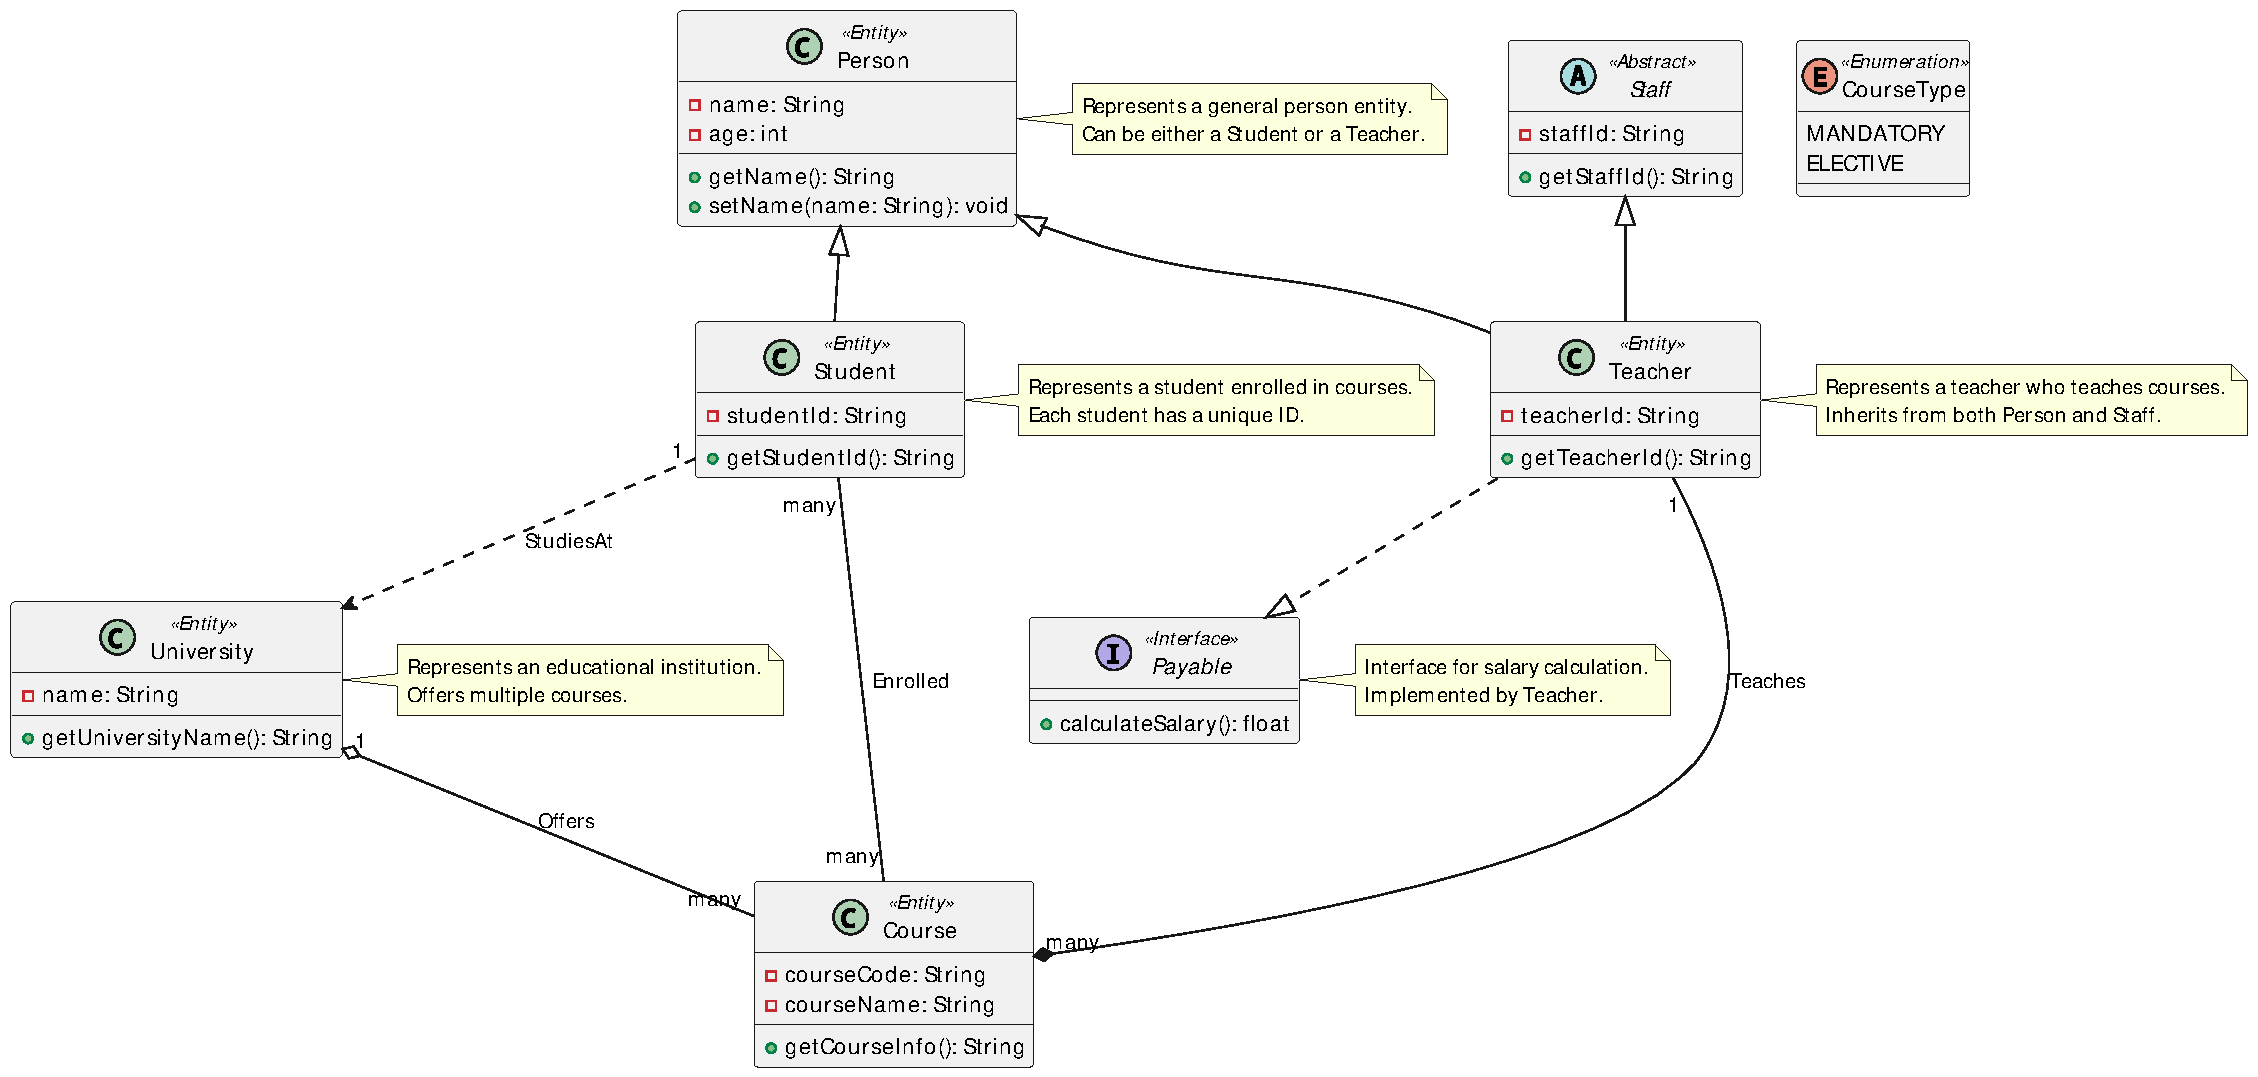
\includegraphics[width=\textwidth]{../figures/out/class_diagram}
	\caption{Class diagram and its features}
	\label{fig:class_diagram}
\end{figure}

\begin{lstlisting}[language=puml, caption={UML class diagram menggunakan PlantUML}]
@startuml
'Define Classes with attributes and methods
class Person <<Entity>> {
	-name: String
	-age: int
	+getName(): String
	+setName(name: String): void
}

class Student <<Entity>> {
	-studentId: String
	+getStudentId(): String
}

class Teacher <<Entity>> {
	-teacherId: String
	+getTeacherId(): String
}

class Course <<Entity>> {
	-courseCode: String
	-courseName: String
	+getCourseInfo(): String
}

class University <<Entity>> {
	-name: String
	+getUniversityName(): String
}

' Abstract Class
abstract class Staff <<Abstract>> {
	-staffId: String
	+getStaffId(): String
}

' Interface
interface Payable <<Interface>> {
	+calculateSalary(): float
}

' Enumeration
enum CourseType <<Enumeration>> {
	MANDATORY
	ELECTIVE
}

' Relationships
Person <|-- Student  
Person <|-- Teacher  
Staff <|-- Teacher   
Teacher ..|> Payable 

University "1" o-- "many" Course  : Offers  
Student "many" -- "many" Course   : Enrolled  
Teacher "1" --* "many" Course    : Teaches  
Student "1" ..> University       : StudiesAt  

' Adding Notes
note right of Person
Represents a general person entity.
Can be either a Student or a Teacher.
end note

note right of Student
Represents a student enrolled in courses.
Each student has a unique ID.
end note

note right of Teacher
Represents a teacher who teaches courses.
Inherits from both Person and Staff.
end note

note right of University
Represents an educational institution.
Offers multiple courses.
end note

note right of Payable
Interface for salary calculation.
Implemented by Teacher.
end note

@enduml
\end{lstlisting}

\subsection{Kelas dan Atribut}
Setiap kelas dalam class diagram direpresentasikan sebagai sebuah kotak yang terdiri dari tiga bagian, yaitu nama kelas, atribut, dan metode. Contoh kelas dalam diagram yang diberikan adalah \texttt{Person}, \texttt{Student}, \texttt{Teacher}, \texttt{Course}, dan \texttt{University}. Atribut dalam kelas ditulis dalam format \texttt{name: type}, seperti berikut:
\begin{lstlisting}[language=puml]
	class Person {
		-name: String
		-age: int
	}
\end{lstlisting}
Simbol \texttt{-} menunjukkan bahwa atribut bersifat \textit{private}, sehingga tidak dapat diakses secara langsung dari luar kelas.

\subsection{Metode dalam Kelas}
Selain atribut, kelas juga memiliki metode yang menunjukkan perilaku atau operasi yang dapat dilakukan oleh objek dari kelas tersebut. Metode dalam UML ditulis dalam format:
\begin{lstlisting}[language=puml]
	+getName(): String
	+setName(name: String): void
\end{lstlisting}
Simbol \texttt{+} menunjukkan bahwa metode bersifat \textit{public}, sehingga dapat diakses dari luar kelas.

\subsection{Hubungan Antar Kelas}
Dalam class diagram, terdapat beberapa jenis hubungan yang menunjukkan keterkaitan antar kelas, yaitu:

\begin{enumerate}
	\item \textbf{Inheritance (Pewarisan)} \\
	Pewarisan dalam UML direpresentasikan dengan panah kosong (\texttt{<|--}) yang menunjukkan bahwa suatu kelas merupakan subclass dari kelas lain. Misalnya, kelas \texttt{Student} dan \texttt{Teacher} mewarisi atribut dan metode dari kelas \texttt{Person}:
	\begin{lstlisting}[language=puml]
		Person <|-- Student  
		Person <|-- Teacher
	\end{lstlisting}
	
	\item \textbf{Association (Asosiasi)} \\
	Asosiasi menunjukkan hubungan antar kelas dalam sistem. Misalnya, hubungan antara \texttt{Student} dan \texttt{Course} dalam diagram menunjukkan bahwa banyak mahasiswa dapat mendaftar ke banyak mata kuliah:
	\begin{lstlisting}[language=puml]
		Student "many" -- "many" Course   : Enrolled
	\end{lstlisting}
	
	\item \textbf{Aggregation (Agregasi)} \\
	Agregasi menunjukkan hubungan "bagian dari" tetapi objek yang dimiliki dapat berdiri sendiri tanpa pemiliknya. Dalam contoh diagram, \texttt{University} memiliki banyak \texttt{Course}, tetapi kursus tetap ada meskipun universitas dihapus:
	\begin{lstlisting}[language=puml]
		University "1" o-- "many" Course  : Offers
	\end{lstlisting}
	
	\item \textbf{Composition (Komposisi)} \\
	Komposisi mirip dengan agregasi, tetapi bagian yang dimiliki tidak dapat berdiri sendiri tanpa pemiliknya. Dalam contoh diagram, \texttt{Teacher} memiliki banyak \texttt{Course}, dan kursus tidak akan ada tanpa pengajar:
	\begin{lstlisting}[language=puml]
		Teacher "1" --* "many" Course    : Teaches
	\end{lstlisting}
	
	\item \textbf{Dependency (Ketergantungan)} \\
	Dependency menunjukkan bahwa suatu kelas bergantung pada kelas lain tetapi tidak memiliki hubungan yang kuat. Misalnya, \texttt{Student} bergantung pada \texttt{University}:
	\begin{lstlisting}[language=puml]
		Student "1" ..> University       : StudiesAt
	\end{lstlisting}
\end{enumerate}

\subsection{Kelas Abstrak dan Interface}
Class diagram juga dapat mencakup kelas abstrak dan antarmuka (\textit{interface}). 

\begin{itemize}
	\item \textbf{Kelas Abstrak} \\
	Kelas abstrak tidak dapat diinstansiasi dan biasanya digunakan sebagai dasar bagi kelas lain. Dalam contoh diagram, \texttt{Staff} merupakan kelas abstrak yang diwarisi oleh \texttt{Teacher}:
	\begin{lstlisting}[language=puml]
		abstract class Staff {
			-staffId: String
			+getStaffId(): String
		}
	\end{lstlisting}
	
	\item \textbf{Interface} \\
	Interface mendefinisikan metode yang harus diimplementasikan oleh kelas yang menggunakannya. Dalam contoh diagram, \texttt{Payable} merupakan interface yang diimplementasikan oleh \texttt{Teacher}:
	\begin{lstlisting}[language=puml]
		interface Payable {
			+calculateSalary(): float
		}
		
		Teacher ..|> Payable
	\end{lstlisting}
\end{itemize}

\subsection{Enumerasi}
Enumerasi (\textit{Enumeration}) adalah tipe data khusus yang berisi sekumpulan nilai tetap. Dalam diagram ini, \texttt{CourseType} adalah enumerasi dengan dua nilai:
\begin{lstlisting}[language=puml]
	enum CourseType {
		MANDATORY
		ELECTIVE
	}
\end{lstlisting}

\subsection{Stereotip}
Stereotip dalam UML digunakan untuk mengklasifikasikan elemen dalam diagram. Dalam contoh diagram, digunakan stereotip seperti berikut:
\begin{itemize}
	\item \texttt{<<Entity>>} untuk kelas seperti \texttt{Person}, \texttt{Student}, dan \texttt{Course}.
	\item \texttt{<<Abstract>>} untuk kelas abstrak \texttt{Staff}.
	\item \texttt{<<Interface>>} untuk antarmuka \texttt{Payable}.
	\item \texttt{<<Enumeration>>} untuk enumerasi \texttt{CourseType}.
\end{itemize}

\subsection{Catatan (Notes)}
Dalam UML, catatan digunakan untuk memberikan informasi tambahan tentang elemen dalam diagram. Misalnya, pada diagram terdapat catatan yang menjelaskan fungsi dari kelas \texttt{Person}:
\begin{lstlisting}[language=puml]
	note right of Person
	Represents a general person entity.
	Can be either a Student or a Teacher.
	end note
\end{lstlisting}

Class diagram adalah alat yang sangat berguna dalam pemodelan perangkat lunak karena memungkinkan pengembang untuk memahami struktur sistem sebelum implementasi. Diagram ini mencakup berbagai elemen seperti kelas, atribut, metode, hubungan antar kelas, serta konsep seperti kelas abstrak, interface, enumerasi, dan catatan untuk dokumentasi tambahan.

\section{Object Diagram}

Object diagram merupakan salah satu diagram struktural dalam Unified Modeling Language (UML) yang digunakan untuk merepresentasikan instance dari kelas pada suatu waktu tertentu. Diagram ini memberikan gambaran bagaimana objek-objek dalam sistem saling berinteraksi dan berhubungan dalam keadaan tertentu.

\begin{figure}[ht]
	\centering
	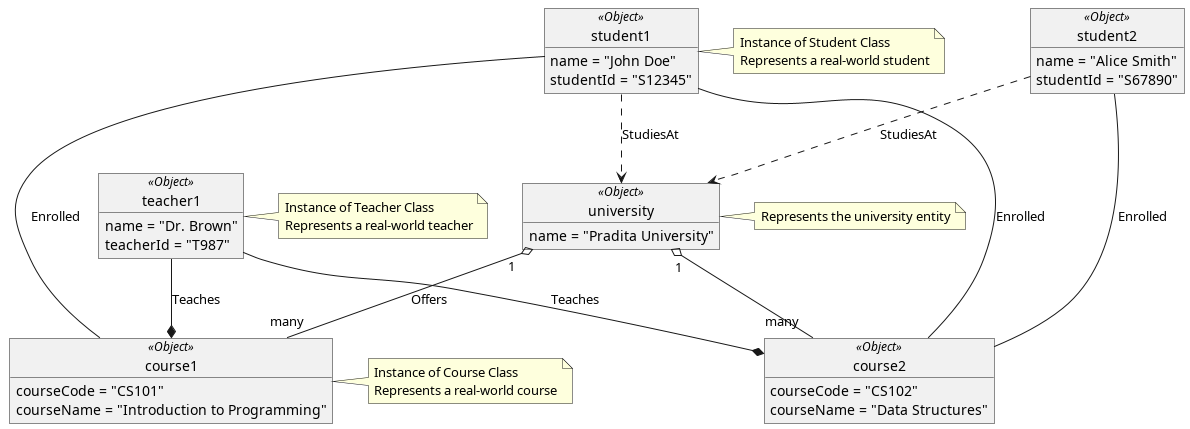
\includegraphics[width=\textwidth]{../figures/out/object_diagram}
	\caption{Object Diagram dan Fitur-fiturnya}
	\label{fig:object_diagram}
\end{figure}

\begin{lstlisting}[language=puml,caption={PlantUML Object Diagram Code}]
	@startuml
	
	' Defining Objects
	object student1 <<Object>> {
		name = "John Doe"
		studentId = "S12345"
	}
	
	object student2 <<Object>> {
		name = "Alice Smith"
		studentId = "S67890"
	}
	
	object course1 <<Object>> {
		courseCode = "CS101"
		courseName = "Introduction to Programming"
	}
	
	object course2 <<Object>> {
		courseCode = "CS102"
		courseName = "Data Structures"
	}
	
	object teacher1 <<Object>> {
		name = "Dr. Brown"
		teacherId = "T987"
	}
	
	object university <<Object>> {
		name = "Pradita University"
	}
	
	' Relationships
	student1 -- course1 : Enrolled
	student1 -- course2 : Enrolled
	student2 -- course2 : Enrolled
	teacher1 --* course1 : Teaches
	teacher1 --* course2 : Teaches
	university "1" o-- "many" course1 : Offers
	university "1" o-- "many" course2
	
	' Dependency Relationship
	student1 ..> university : StudiesAt
	student2 ..> university : StudiesAt
	
	' Notes for explanation
	note right of student1
	Instance of Student Class
	Represents a real-world student
	end note
	
	note right of course1
	Instance of Course Class
	Represents a real-world course
	end note
	
	note right of teacher1
	Instance of Teacher Class
	Represents a real-world teacher
	end note
	
	note right of university
	Represents the university entity
	end note
	
	@enduml
\end{lstlisting}


\subsection{Objek dan Atributnya}
Objek dalam object diagram merepresentasikan instance spesifik dari suatu kelas dalam sistem. Objek dalam UML ditulis dengan format:
\begin{lstlisting}[language=puml]
	object student1 <<Object>> {
		name = "John Doe"
		studentId = "S12345"
	}


\end{lstlisting}
Objek \texttt{student1} adalah instance dari kelas \texttt{Student} dengan nilai atribut spesifik. Setiap objek memiliki nama yang menunjukkan bahwa objek tersebut merupakan realisasi dari suatu kelas.

\subsection{Hubungan Antar Objek}
Seperti dalam class diagram, object diagram juga menggambarkan hubungan antar objek dalam sistem. Beberapa hubungan yang dapat muncul dalam diagram objek antara lain:

\begin{enumerate}
	\item \textbf{Association (Asosiasi)} \\
	Asosiasi menunjukkan hubungan antara dua objek tanpa menunjukkan kepemilikan. Contoh pada diagram adalah hubungan antara \texttt{student1} dan \texttt{course1} yang menunjukkan bahwa mahasiswa terdaftar pada suatu kursus:
	\begin{lstlisting}[language=puml]
		student1 -- course1 : Enrolled
	\end{lstlisting}
	
	\item \textbf{Aggregation (Agregasi)} \\
	Agregasi menunjukkan bahwa satu objek merupakan bagian dari objek lain, tetapi masih dapat berdiri sendiri. Contohnya adalah \texttt{university} yang memiliki banyak \texttt{course}, tetapi kursus tetap bisa ada meskipun universitas tidak ada:
	\begin{lstlisting}[language=puml]
		university "1" o-- "many" course1 : Offers
	\end{lstlisting}
	
	\item \textbf{Composition (Komposisi)} \\
	Komposisi menunjukkan bahwa satu objek tidak dapat berdiri sendiri tanpa objek pemiliknya. Contohnya adalah hubungan antara \texttt{teacher1} dan \texttt{course1}, yang menunjukkan bahwa kursus tidak bisa ada tanpa seorang pengajar:
	\begin{lstlisting}[language=puml]
		teacher1 --* course1 : Teaches
	\end{lstlisting}
	
	\item \textbf{Dependency (Ketergantungan)} \\
	Dependency menunjukkan bahwa satu objek bergantung pada objek lain, tetapi tidak memiliki hubungan yang kuat. Contohnya adalah hubungan antara \texttt{student1} dan \texttt{university}:
	\begin{lstlisting}[language=puml]
		student1 ..> university : StudiesAt
	\end{lstlisting}
\end{enumerate}

\subsection{Stereotip dalam Object Diagram}
Stereotip digunakan untuk memberikan klasifikasi tambahan pada objek dalam diagram UML. Dalam object diagram, digunakan stereotip \texttt{<<Object>>} untuk menandai bahwa elemen tersebut merupakan instance dari suatu kelas:
\begin{lstlisting}[language=puml]
	object student1 <<Object>> {
		name = "John Doe"
		studentId = "S12345"
	}
\end{lstlisting}

\subsection{Catatan (Notes)}
Catatan digunakan untuk memberikan informasi tambahan mengenai suatu elemen dalam object diagram. Contohnya adalah catatan yang menjelaskan objek \texttt{student1}:
\begin{lstlisting}[language=puml]
	note right of student1
	Instance of Student Class
	Represents a real-world student
	end note
\end{lstlisting}
Catatan ini menjelaskan bahwa objek \texttt{student1} adalah instance dari kelas \texttt{Student} dan mewakili seorang mahasiswa nyata dalam sistem.

Object diagram adalah alat yang berguna dalam pemodelan perangkat lunak karena memberikan gambaran bagaimana objek dalam sistem berinteraksi pada suatu titik waktu tertentu. Diagram ini mencakup berbagai elemen seperti objek, atribut, hubungan antar objek, serta konsep seperti asosiasi, agregasi, komposisi, dependency, stereotip, dan catatan untuk dokumentasi tambahan.


\section{Component Diagram}

Component diagram merupakan salah satu diagram struktural dalam Unified Modeling Language (UML) yang digunakan untuk merepresentasikan komponen-komponen dalam suatu sistem perangkat lunak beserta hubungan antar komponen tersebut. Diagram ini berguna untuk memahami bagaimana komponen dalam sistem berinteraksi satu sama lain dan bagaimana layanan-layanan tertentu disediakan dan digunakan.

\begin{figure}[ht]
	\centering
	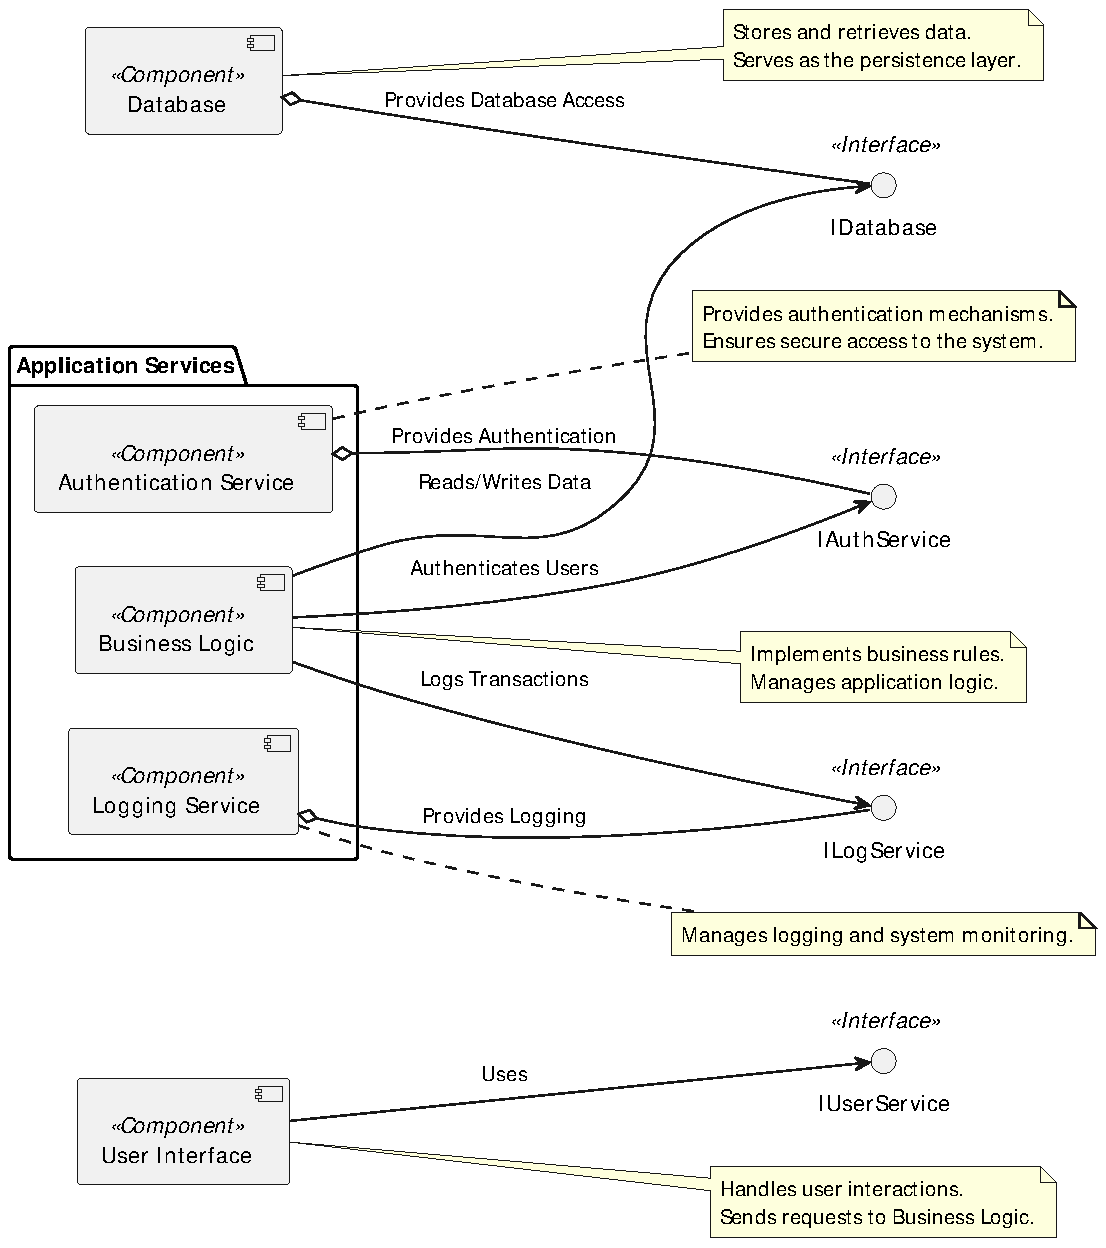
\includegraphics[width=.9\textwidth]{../figures/out/component_diagram}
	\caption{Component Diagram dan Fitur-fiturnya}
	\label{fig:component_diagram}
\end{figure}

\begin{lstlisting}[language=puml,caption={PlantUML Component Diagram Code}]
	@startuml
	
	' Force vertical layout
	left to right direction
	
	' Define components inside the package
	package "Application Services" {
		component "Business Logic" <<Component>> as BL
		component "Authentication Service" <<Component>> as Auth
		component "Logging Service" <<Component>> as Log
	}
	
	' Define other components
	component "User Interface" <<Component>> as UI
	component "Database" <<Component>> as DB
	
	' Define interfaces
	interface "IUserService" <<Interface>> as IUserService
	interface "IDatabase" <<Interface>> as IDatabase
	interface "IAuthService" <<Interface>> as IAuthService
	interface "ILogService" <<Interface>> as ILogService
	
	' Component dependencies
	UI --> IUserService : Uses
	BL --> IDatabase : Reads/Writes Data
	BL --> IAuthService : Authenticates Users
	BL --> ILogService : Logs Transactions
	Auth o-- IAuthService : Provides Authentication
	DB o-- IDatabase : Provides Database Access
	Log o-- ILogService : Provides Logging
	
	' Notes explaining components
	note right of UI
	Handles user interactions.
	Sends requests to Business Logic.
	end note
	
	note right of BL
	Implements business rules.
	Manages application logic.
	end note
	
	note right of DB
	Stores and retrieves data.
	Serves as the persistence layer.
	end note
	
	note right of Auth
	Provides authentication mechanisms.
	Ensures secure access to the system.
	end note
	
	note right of Log
	Manages logging and system monitoring.
	end note
	
	@enduml
\end{lstlisting}


\subsection{Komponen dalam Diagram Komponen}
Komponen dalam UML direpresentasikan sebagai unit mandiri yang memiliki antarmuka dan dapat digunakan kembali. Setiap komponen dalam diagram ini dideklarasikan menggunakan stereotip \texttt{<<Component>>}. Contohnya:
\begin{lstlisting}[language=puml]
	component "User Interface" <<Component>> as UI
	component "Business Logic" <<Component>> as BL
	component "Database" <<Component>> as DB
\end{lstlisting}
Komponen \texttt{User Interface} berfungsi sebagai lapisan interaksi dengan pengguna, sementara \texttt{Business Logic} menangani aturan bisnis, dan \texttt{Database} bertindak sebagai penyimpanan data.

\subsection{Antarmuka dalam Diagram Komponen}
Antarmuka (\textit{interface}) digunakan untuk menentukan layanan yang disediakan atau diperlukan oleh suatu komponen. Antarmuka dalam UML dinyatakan menggunakan stereotip \texttt{<<Interface>>}. Contoh definisi antarmuka:
\begin{lstlisting}[language=puml]
	interface "IUserService" <<Interface>> as IUserService
	interface "IDatabase" <<Interface>> as IDatabase
\end{lstlisting}
Antarmuka ini digunakan untuk mendeklarasikan kontrak layanan yang harus dipenuhi oleh komponen.

\subsection{Hubungan Antar Komponen}
Diagram komponen menunjukkan berbagai hubungan antara komponen dalam sistem. Beberapa jenis hubungan yang umum digunakan dalam diagram ini meliputi:

\begin{enumerate}
	\item \textbf{Dependency (Ketergantungan)} \\
	Ketergantungan menunjukkan bahwa satu komponen menggunakan layanan dari komponen lain. Dalam contoh berikut, \texttt{User Interface} bergantung pada layanan \texttt{IUserService}:
	\begin{lstlisting}[language=puml]
		UI --> IUserService : Uses
	\end{lstlisting}
	
	\item \textbf{Provided Interface (Antarmuka yang Disediakan)} \\
	Komponen yang menyediakan layanan akan menunjukkan antarmuka yang disediakannya menggunakan simbol \texttt{o--}. Contohnya, komponen \texttt{Database} menyediakan layanan \texttt{IDatabase}:
	\begin{lstlisting}[language=puml]
		DB o-- IDatabase : Provides Database Access
	\end{lstlisting}
	
	\item \textbf{Required Interface (Antarmuka yang Dibutuhkan)} \\
	Komponen yang membutuhkan layanan dari komponen lain akan menggunakan simbol \texttt{-->}. Contoh berikut menunjukkan bahwa komponen \texttt{Business Logic} memerlukan layanan dari \texttt{IDatabase}:
	\begin{lstlisting}[language=puml]
		BL --> IDatabase : Reads/Writes Data
	\end{lstlisting}
\end{enumerate}

\subsection{Pengelompokan Komponen dengan Paket}
Dalam sistem besar, komponen dapat dikelompokkan ke dalam paket untuk menunjukkan bagian-bagian modular dari sistem. Dalam diagram ini, beberapa komponen dikelompokkan ke dalam paket \texttt{Application Services}:
\begin{lstlisting}[language=puml]
	package "Application Services" {
		component "Business Logic" <<Component>> as BL
		component "Authentication Service" <<Component>> as Auth
		component "Logging Service" <<Component>> as Log
	}
\end{lstlisting}
Pengelompokan ini membantu dalam memahami arsitektur sistem secara lebih terstruktur.

\subsection{Catatan (Notes) dalam Diagram Komponen}
Catatan digunakan untuk memberikan informasi tambahan mengenai suatu komponen atau hubungan antar komponen dalam diagram. Misalnya, berikut adalah catatan yang menjelaskan fungsi dari komponen \texttt{User Interface}:
\begin{lstlisting}[language=puml]
	note right of UI
	Handles user interactions.
	Sends requests to Business Logic.
	end note
\end{lstlisting}
Catatan ini membantu menjelaskan peran setiap komponen dalam sistem secara lebih rinci.


Component diagram adalah alat yang sangat berguna dalam pemodelan perangkat lunak karena memungkinkan desainer untuk memahami bagaimana komponen dalam sistem berinteraksi satu sama lain. Diagram ini mencakup berbagai elemen seperti komponen, antarmuka, hubungan antar komponen, pengelompokan dalam paket, serta catatan untuk dokumentasi tambahan.


\section{Deployment Diagram dan Fitur-fiturnya}

Deployment Diagram merupakan salah satu diagram dalam Unified Modeling Language (UML) yang digunakan untuk memodelkan arsitektur fisik dari sistem perangkat lunak. Diagram ini menunjukkan bagaimana komponen perangkat lunak dipetakan ke perangkat keras serta bagaimana komunikasi antara berbagai elemen dilakukan.

\begin{figure}[ht]
	\centering
	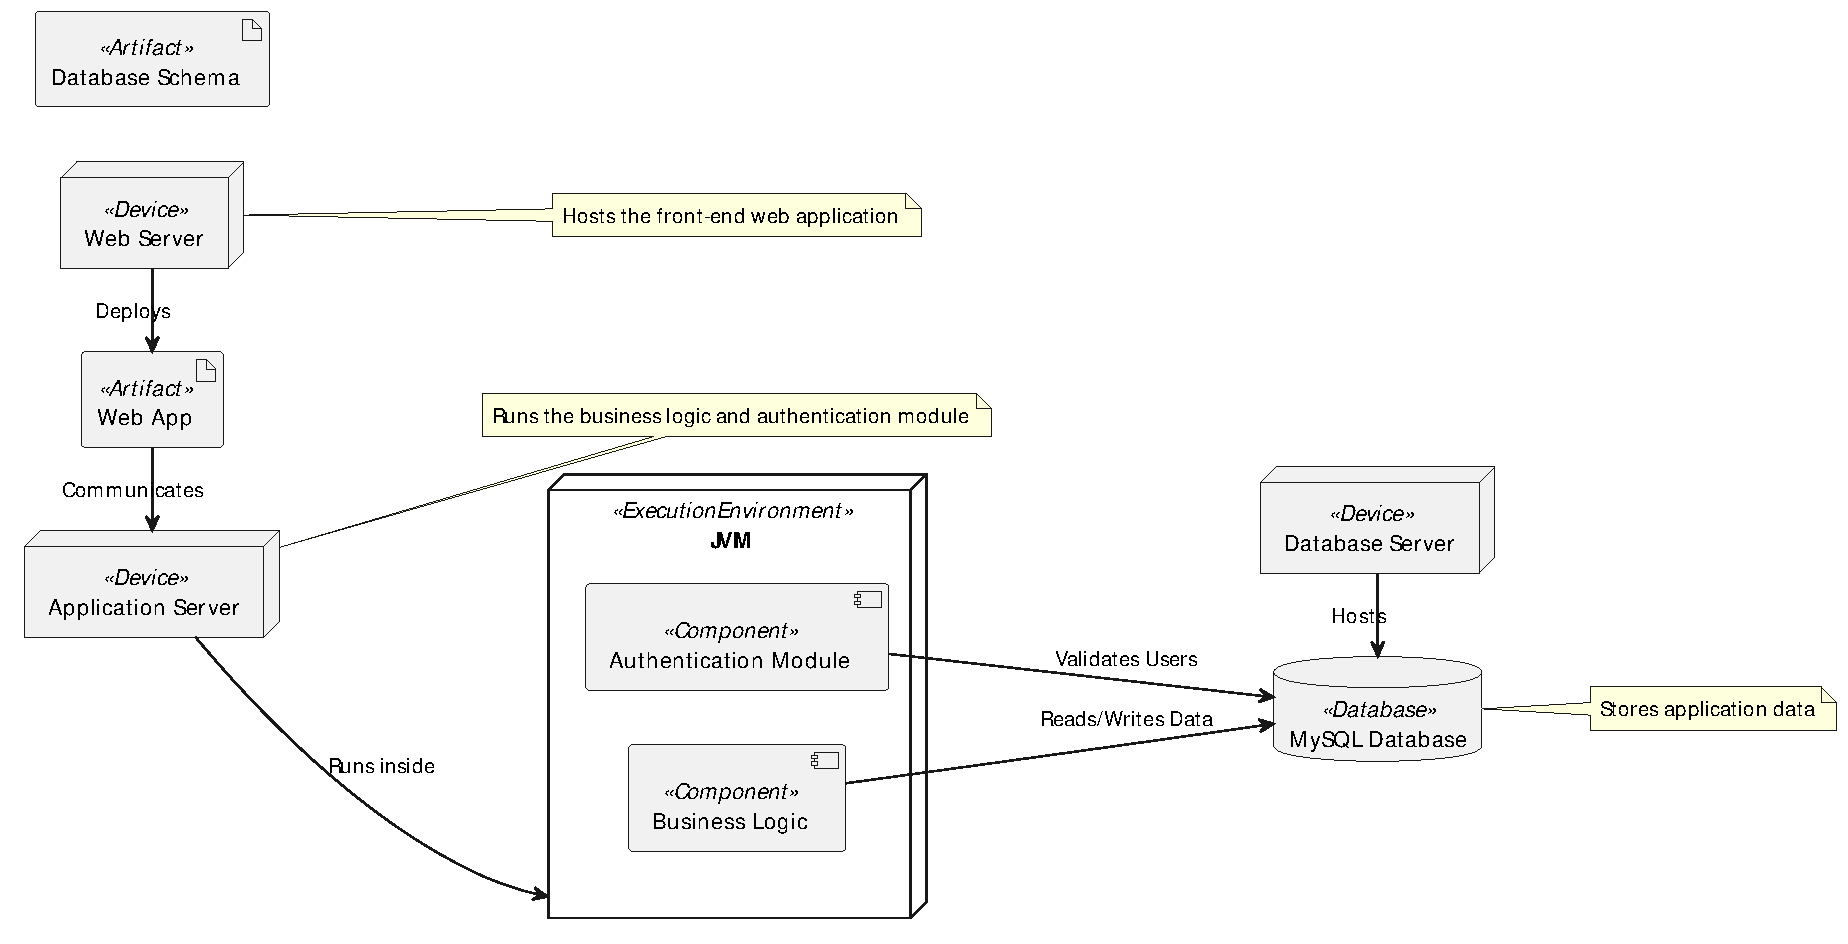
\includegraphics[width=\textwidth]{../figures/out/deployment_diagram}
	\caption{Deployment Diagram dan Fitur-fiturnya}
	\label{fig:deployment_diagram}
\end{figure}



\subsection{Node dalam Deployment Diagram}
Node (\textit{simpul}) adalah elemen utama dalam deployment diagram yang merepresentasikan perangkat keras atau lingkungan eksekusi yang digunakan untuk menjalankan komponen perangkat lunak. Node dalam UML dapat memiliki stereotip seperti \texttt{<<Device>>} dan \texttt{<<ExecutionEnvironment>>}.

\begin{lstlisting}[language=puml,caption={Contoh Definisi Node dalam Deployment Diagram}]
	node "Web Server" <<Device>> as WebServer
	node "Application Server" <<Device>> as AppServer
	node "Database Server" <<Device>> as DBServer
\end{lstlisting}
Dalam contoh di atas, terdapat tiga node utama yang mewakili server tempat sistem dijalankan, yaitu Web Server, Application Server, dan Database Server.

\subsection{Lingkungan Eksekusi (Execution Environment)}
Lingkungan eksekusi (\textit{Execution Environment}) digunakan untuk merepresentasikan platform perangkat lunak tempat komponen dijalankan, seperti JVM (Java Virtual Machine), container Docker, atau runtime lainnya.

\begin{lstlisting}[language=puml,caption={Contoh Execution Environment dalam Deployment Diagram}]
	node "JVM" <<ExecutionEnvironment>> as JVM {
		component "Business Logic" <<Component>> as BL
		component "Authentication Module" <<Component>> as Auth
	}
\end{lstlisting}
Dalam contoh di atas, lingkungan eksekusi \texttt{JVM} berada di dalam \texttt{Application Server} dan digunakan untuk menjalankan komponen seperti \texttt{Business Logic} dan \texttt{Authentication Module}.

\subsection{Artefak dalam Deployment Diagram}
Artefak (\textit{Artifact}) dalam deployment diagram merepresentasikan entitas fisik dari perangkat lunak, seperti file aplikasi web, database schema, atau pustaka perangkat lunak yang di-deploy.

\begin{lstlisting}[language=puml,caption={Contoh Artefak dalam Deployment Diagram}]
	artifact "Web App" <<Artifact>> as WebApp
	artifact "Database Schema" <<Artifact>> as DBSchema
\end{lstlisting}
Pada contoh di atas, terdapat dua artefak: \texttt{Web App}, yang merepresentasikan aplikasi web yang dijalankan di server, dan \texttt{Database Schema}, yang merepresentasikan skema database.

\subsection{Database dalam Deployment Diagram}
Deployment diagram juga dapat menyertakan elemen \texttt{<<Database>>} untuk menunjukkan sistem penyimpanan data yang digunakan dalam arsitektur perangkat lunak.

\begin{lstlisting}[language=puml,caption={Contoh Database dalam Deployment Diagram}]
	database "MySQL Database" <<Database>> as MySQLDB
\end{lstlisting}
Dalam diagram ini, \texttt{MySQL Database} berfungsi sebagai penyimpanan utama untuk aplikasi.

\subsection{Hubungan Antar Komponen dalam Deployment Diagram}
Deployment diagram mendukung beberapa jenis hubungan antar elemen, termasuk:

\begin{itemize}
	\item \textbf{Deployment (Pendeployan)} \\
	Menunjukkan bahwa suatu artefak dideploy ke dalam suatu node.
	\begin{lstlisting}[language=puml]
		WebServer -right-> WebApp : Deploys
	\end{lstlisting}
	
	\item \textbf{Communication (Komunikasi)} \\
	Menunjukkan bagaimana komponen berkomunikasi satu sama lain.
	\begin{lstlisting}[language=puml]
		WebApp -right-> AppServer : Communicates
	\end{lstlisting}
	
	\item \textbf{Hosting (Hosting)} \\
	Menunjukkan bahwa suatu komponen berjalan di dalam suatu lingkungan eksekusi.
	\begin{lstlisting}[language=puml]
		AppServer -down-> JVM : Runs inside
	\end{lstlisting}
\end{itemize}

\subsection{Catatan (Notes) dalam Deployment Diagram}
Deployment diagram sering menyertakan catatan untuk memberikan penjelasan tambahan mengenai elemen diagram.

\begin{lstlisting}[language=puml,caption={Contoh Catatan dalam Deployment Diagram}]
	note right of WebServer
	Hosts the front-end web application
	end note
\end{lstlisting}

Catatan ini membantu dalam memberikan deskripsi yang lebih jelas mengenai peran masing-masing komponen dalam diagram.

Deployment diagram adalah alat penting dalam rekayasa perangkat lunak yang memungkinkan pengembang untuk memahami bagaimana sistem diimplementasikan pada infrastruktur fisik. Diagram ini mencakup elemen-elemen seperti node (\textit{device, execution environment}), artefak, database, serta berbagai jenis hubungan seperti \textit{deployment}, \textit{communication}, dan \textit{hosting}. 

\section{Referensi}
Untuk pembelajaran lebih mendalam mengenai UML, silahkan kunjungi tautan berikut: \url{https://www.uml-diagrams.org/}.


